\documentclass{article}

% ------ TEMPLATE ------ %

% ---------------------- %

% ------ PACKAGES ------ %

\usepackage{charter}
\usepackage{geometry}
\usepackage{amsmath}
\usepackage{amssymb}
\usepackage{float}
\usepackage{graphicx}
\usepackage{tabularx}
\usepackage{array}
\usepackage{subcaption}
\usepackage{enumitem}
\usepackage{titlesec}
\usepackage{hyperref}
\usepackage{xcolor}
\usepackage{pifont}
\usepackage{fancyvrb}
\usepackage{listings}
\usepackage{multirow}
\usepackage{ulem}
\usepackage{minted}

% ---------------------- %

% ------ GENERALS ------ %

\setlist[itemize]{label=\scriptsize\textbullet}
\setlist[itemize]{noitemsep, topsep=1pt}
\setlist[enumerate]{noitemsep, topsep=1pt}

\titleformat{\chapter}[hang]
{\normalfont\huge\bfseries}{\thechapter}{1em}{}
\titleformat{\subsubsection}{\large\bfseries}{\thesubsubsection}{1em}{}

% ---------------------- %

% ------- COLORS ------- %

\hypersetup{
    colorlinks=true,
    linkcolor=blue!50!black,
    urlcolor=blue,
    citecolor=blue,
    pdfborder={0 0 0}
}

% ---------------------- %

% ------ COMMANDS ------ %

\newcommand{\vmark}{\textcolor{teal}{\ding{51}}}
\newcommand{\xmark}{\textcolor{red!70!black}{\ding{55}}}
\newcommand{\newpar}[0]{\vspace{2mm}\noindent}
\newcommand{\htitle}[1]{\newpar\textbf{#1 -}}
\newcommand{\ititle}[1]{\newpar\hspace{1em}\textbf{#1}}
\newcommand{\hyperlabel}[1]{\hypertarget{#1}\phantomsection\label{#1}}
\newcommand{\hyperitem}[2]{\item \hyperlink{#1}{#2}\leaders\hbox to 0.8em{\hss.\hss}\hfill\hbox to 1.8em{\hss\pageref{#1}}}
\newcommand{\stdtilde}[0]{\raise.17ex\hbox{$\scriptstyle\sim$}}
\newcommand{\xor}[0]{\char`\^}
\newcommand{\saveformula}[2]{\newbox{#1}\savebox{#1}{#2}}
\newcommand{\useformula}[1]{\usebox{#1}}

% ---------------------- %

\begin{document}

% -------- HEAD -------- %

\pagenumbering{gobble}

\begin{center}

	\fontsize{20pt}{30pt}\selectfont
	Well MEing

	\vspace{2cm}

	\fontsize{25pt}{45pt}\selectfont
	\textbf{Developer Guide}

	\vfill

	\fontsize{12pt}{18pt}\selectfont
	Matteo Bettiati \\
	Lorenzo Bianchi \\
	Alessio Caggiano \\
	Francesco Ostidich \\
	Denis Sanduleanu \\

	\vspace{1cm}

	\today \\
	\vspace{12pt}
	Version: 0.1
	\normalsize

\end{center}

\newpage
\pagenumbering{arabic}
\tableofcontents
\newpage

% ---------------------- %

% -------- BODY -------- %

\section{Introduction}

This document provides a low level description of the system architecture, outlining the deployment structure, code organization, and exposed endpoints.
It also showcases the strategies an techniques chosen for designing the AI modules.

The goal is to ensure maintainability, scalability, and clarity for future development.
Finally, contributions from each team member are summarized.

\section{Deployment view}

The system follows a cloud-based, serverless architecture, with the frontend on mobile platforms, and functionalities hosted on Firebase.

The client is a Swift-based iOS application running on iPhones, responsible for the user interface and local interactions.

All backend services are hosted on Firebase, leveraging its functions, written in Python, to handle endpoints and AI-related processing.
Firebase Authentication manages user login and access control, while a NoSQL realtime database allow for storing and retrieving application data.
For AI capabilities, the backend integrates with Google Cloud's Vertex AI and Generative AI services to handle inference and model execution tasks.

\begin{figure}[H]
	\centering
	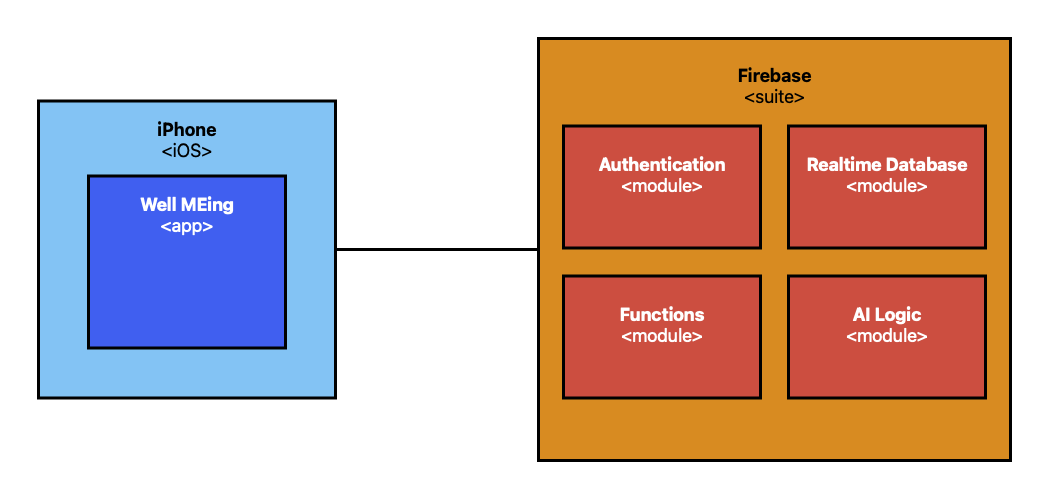
\includegraphics[width=0.6\textwidth]{images/deployment-view.png}
\end{figure}

\section{Code structure}

The following sections describe the project folder trees for both the client Swift app and the Firebase Python functions (with focus on the hosted code for running the AI).

\subsection{Client}

\begin{verbatim}
Well-MEing/
  - Models/
  - Services/
  - Views/
      - Branded/
      - Contents/
      - Elements/
      - InputSelectors/
      - InputTypes/
      - Sections/
\end{verbatim}

\newpar
The client project contains a little \textbf{Models} folder in which the main objects used throughout the client codebase are defined.
These resembles either DB entities or DTOs, which, in general, coincide.
The main model class is the \verb|UserCache|, which defines a shared static object that is the entrypoint for reaching all user's fetched information, like habits, reports, or personal data.

\newpar
The \textbf{Services} folder mainly contains the code used to express the logic executing on the client.
In particular, here is found the code for enabling authentication, making requests to the backend, processing past data, enabling the text-to-speech recognition, and importing data from Apple Health.

\newpar
Finally, the \textbf{View} folder, being the client a frontend application, contains all the SwiftUI structs which compose the presentation layer.

Subfolders helps to organize view components based on their purposes.

The three main app sections (dashboard, assistant, progress) are defined in the \textbf{Sections} folder.
The other main pages that are placed above in the navigation stack base are found in the \textbf{Contents} folder.
General little components are found in the \textbf{Elements} folder, whereas others that are more theme-related are found in the \textbf{Branded} one.
The metric input formats may have slightly different definitions, as they can be used either as simple type previews in the habit creation panel, or as concrete selectors for the habit logging; they are thus organized separately in two dedicated folders.

\subsection{Server}

\begin{verbatim}
functions/
  - ai/
      - ai_setup/
      - ai_tools/
          - schemas/
          - tools/
      - auxiliary/
      - dto/
      - report/
      - test/
      - ui_schema/
  - db/
\end{verbatim}

\newpar
The server folder contains the code deployed to Firebase as Cloud Functions endpoints.
It is organized into two main logic blocks:

\begin{itemize}
	\item the AI logic, which initializes LLM connections and sets up the AI agent for text-to-action recognition and report generation;
	\item the DB logic, which defines the endpoints used to validate and update entries in the Firebase Database upon receiving creation or deletion requests.
\end{itemize}

\newpar 

\subsubsection{AI Core Setup}

The \texttt{ai\_setup} folder serves as the central configuration hub for the AI logic. Within it, \texttt{graph\_components.py} defines the key graph elements such as node types, state transitions, token usage monitoring, and conditional logic for tool execution. The core logic that governs how the graph is built and executed resides in \texttt{graph\_logic.py}, which initializes the state machine and launches the flow using LangGraph. The integration with the VertexAI platform is handled by \texttt{llm\_setup.py}, which authenticates the LLM and binds it to a defined set of tools using LangChain conventions.

\subsubsection{Tooling and Schema Management}

The implementation of AI tools is structured under the \texttt{ai\_tools} directory. This is further divided into two components: the \texttt{tools} subfolder contains the functional definitions of the actions the LLM can invoke (e.g., \texttt{create\_habit}, \texttt{insert\_habit\_data}), while the \texttt{schema} subfolder holds the input schemas for each tool. These schemas are defined using Pydantic and serve a dual purpose: they validate inputs both before and during execution, and they inform the LLM about the format and semantics expected for each parameter.

\subsubsection{Auxiliary Processing and Key Management}

Support functions that enhance readability and usability of the AI outputs are located in the \texttt{auxiliary} folder. This module includes transformations that reformat raw JSON outputs from the tools into a more structured and user-friendly layout, suitable for frontend rendering. To maintain consistency across modules, the \texttt{json\_keys} module defines all key names through centralized enum classes, reducing duplication and potential mismatches.

\subsubsection{Context Management and Utilities}

General-purpose utilities are defined in \texttt{utils.py}, with a notable feature being the \texttt{ContextManager} class. This class handles the conversion of the context dictionary into a natural language description, which is embedded into the LLM prompt. It also supports dynamic updates and validation control during graph execution, playing a key role in keeping the agent state aligned with the application's logic.

\subsubsection{Data Transfer and Interface Alignment}

Input and output validation is handled by a series of Data Transfer Objects (DTOs), housed in the \texttt{dto} folder. These objects guarantee that external data entering or exiting the system adheres to a predefined schema. In parallel, the \texttt{ui\_schema} folder defines output constraints specific to the user interface, ensuring that the final JSON responses generated by the AI are fully compatible with the frontend display logic.

% TODO: lolly scrivi qua 1

\newpar
The DB section contains only the definitions of the functions used to update the DB.
Since no particular logic is required, all of its code is found directly in the root of the \textbf{db} folder.

\section{Endpoints}

The following endpoints are exposed by Firebase as Cloud Functions.
They use standard HTTP status codes for success and error handling.

\subsection{generate\_report}

The \textbf{POST} request accepts an list of habit (including a subset of the history submissions) and optional user information (name and bio).
This data is sent to the LLM, which generates a personalized user report in Markdown format, which is then returned.

\subsection{process\_speech}

The \textbf{POST} request accepts a speech transcript (text) and an optional list of habit (including a subset of the history submissions).
The backend's LLM analyzes the content and returns two sets of actions (operation previews): new habit creations and habit submissions.
These are not automatically executed and require user confirmation.

\subsection{create\_habit}

The \textbf{POST} request accepts an habit definition and creates it in the database.
The habit name (ID) must be added as a URL variable.
All metrics must match a valid input type.

\subsection{delete\_habit}

The \textbf{DELETE} request deletes the specified habit from the database.
The habit name (ID) must be added as a URL variable.

\subsection{create\_submission}

The \textbf{POST} request accepts a submission for a given habit and stores it in the database.
The habit name (ID) must be added as a URL variable.
The provided metrics must match the habit's definition.

\subsection{delete\_submission}

The \textbf{DELETE} request deletes the specified submission from the database.
The habit name (ID) and submission ID must be added as a URL variable.

\subsection{delete\_report}

The \textbf{DELETE} request deletes the specified report from the database.
The report date (ID) must be added as a URL variable.

\subsection{update\_name}

The \textbf{POST} request accepts a new name and creates/updates the corresponding value in the database.
Valid names are 4–32 characters long and may contain only letters and spaces.

\newpar
The \textbf{DELETE} request deletes the user's name value in the database.

\subsection{update\_bio}

The \textbf{POST} request accepts a new bio and creates/updates the corresponding value in the database.
Valid bios are 8–256 characters long.

\newpar
The \textbf{DELETE} request deletes the user's bio value in the database.

\section{AI Design}

\subsection{Speech recognition}

\subsubsection{Entry Point and Input Handling}
The system's main entry point is the \texttt{process\_speech} function, which receives HTTPS requests comprising a user’s spoken command as a string (\texttt{speech}) and a dictionary representing the current habit-tracking state (\texttt{context}). Upon receiving the request, the user ID is extracted to track token consumption and enforce usage limitations if necessary.

\subsubsection{Validation and Prompt Preparation}
Input data is initially validated through a custom \texttt{InputDTO}. Following this, the \texttt{speech} and a natural language description of the \texttt{context} are concatenated with a predefined startup prompt. This composite prompt is passed to a LangGraph-powered agent configured with the VertexAI Gemini 2.0 Flash Lite model.

\subsubsection{Tool-Constrained Agent Architecture}
The agent is strictly constrained to interact solely via tool invocations, as enforced by LangGraph and LangChain. Natural language responses are disallowed, ensuring deterministic, structured behavior. The graph architecture enables the agent to call tools such as \texttt{create\_habit} and \texttt{insert\_habit\_data}, each defined with Pydantic schemas. These schemas include detailed validation rules and field descriptions, allowing the model to infer expected input values accurately.

\subsubsection{Error Handling and Output Aggregation}
Tool outputs are automatically checked for errors. If a response fails validation, the agent is reprompted to generate revised inputs. Once valid outputs are obtained, they are reformatted into a consistent JSON schema. Each result is either inserted or appended to an aggregated output JSON object.

\subsubsection{Finalization and Response Delivery}
The loop is terminated by invoking the \texttt{final\_answer} utility tool, which finalizes the constructed output. This output JSON undergoes a final validation phase via an \texttt{OutputDTO}. Upon successful validation, token usage is updated, and the response is returned to the client.

\subsection{Report generation}

In order to create personalized, insightful weekly reports for users based on their tracked habit data, the process involves intelligent data summarization, semantic context retrieval using vector embeddings, and structured content generation by a powerful AI model.

The report generation system provides a robust and intelligent solution for delivering personalized user feedback.
By transforming raw data into meaningful context and leveraging the advanced generative capabilities of Gemini Pro with strict output formatting, the system can produce high-quality, engaging, and actionable wellness reports automatically.

\subsubsection{Architecture}

The system is architected as a serverless backend running on Google Cloud.
The primary components are the following.

\begin{itemize}
	\item Firebase Cloud Function: an HTTP-triggered endpoint (\verb|generate_report|) that serves as the main entry point for the report generation request.
	\item Data processing and embedding module: a set of Python functions responsible for converting raw, time-series user data into contextually relevant text chunks.
	\item Vertex AI’s Gemini Pro model: the core AI engine that takes the processed context and generates a human-readable, structured report.
	\item Firebase Realtime Database: used for storing user data, including habit history, and for saving the final generated reports.
\end{itemize}

\subsubsection{Data processing and context generation}

To provide the AI with the most relevant information without overwhelming it, a multi-step data processing and retrieval pipeline ensures the final report remains focused on recent and meaningful events.
The process begins by transforming raw user data (specifically, historical records for each habit) into concise and descriptive text blocks.
The \verb|extract_habit_chunks| function performs this transformation; it

\begin{enumerate}
	\item calculates summary statistics for all associated metrics (e.g., average, minimum, maximum),
	\item extracts the most recent user-provided notes,
	\item combines the habit’s goal, description, metric summaries, and recent notes into a single, formatted string.
\end{enumerate}

Instead of feeding all historical data to the AI, which would be inefficient and counterproductive, a semantic search mechanism is applied in order to retrieve only the most relevant information for a weekly summary.
Each chunk is converted into a vector using the \verb|text-embedding-004| model, which encodes the semantic meaning of the text into a high-dimensional numerical space.
A predefined query is also embedded into a vector, in order to better guide the search.

To determine relevance, the cosine similarity is computed between the query vector and each habit chunk vector.
This method identifies which chunks are most semantically aligned with the query.
The top-matching chunks (i.e., the most semantically relevant to the query) are then selected and passed as the primary context to the AI.
This retrieval step is performed in the \verb|get_top_chunks| function.

\subsubsection{Prompting the report generation}

Via the \verb|generate_structured_report| function, with the most relevant context identified, the system calls the Gemini Pro model.

A detailed system instruction is provided to the model.
This is a critical step that constrains the AI’s output to meet our exact requirements.
The prompt defines the following rules.

\begin{itemize}
	\item Structure and formatting: specifies the required sections (e.g., Overview, Insights, Suggestions) and the use of Markdown and emojis.
	\item Content rules: sets constraints on the title (e.g., max length, specificity level) and content.
	\item Tone of voice: instructs the model to be friendly, professional, and supportive.
	\item Injected context: the dynamically retrieved "history summary" from the previous steps is injected directly into the prompt.
\end{itemize}

To ensure reliable, machine-readable output, the model is configured to return its response as a JSON object that adheres to a predefined Pydantic schema (\verb|ReportStructure|).
This eliminates the need for fragile text parsing and guarantees the presence of the title and content fields.

\begin{verbatim}
class ReportStructure(BaseModel):
    title: str
    content: str
\end{verbatim}

\subsubsection{Database interaction}

Once the report is successfully generated by the AI, the final steps involve persisting the data and scheduling the next report.
The \verb|save_report_to_db| function performs two key actions in the Firebase Realtime Database.

\begin{enumerate}
	\item It saves the newly generated report (title and content) under the user’s ID with the current timestamp (\verb|/users/{user_id}/reports/{timestamp}|).
	\item It calculates the date for the next report (7 days in the future) and updates the \verb|newReportDate| field in the user’s profile (\verb|/users/{user_id}/|).
\end{enumerate}

\section{Contributions}

Each group member contributed substantially and nearly equally to the overall development of the project.
All members actively participated in the design phase and in key decisions across the main areas of the project: interaction with the LLM, Firebase backend setup, API endpoint definitions, client implementation, and documentation.

To better leverage individual strengths and ensure high focus on specific tasks, responsibilities were distributed while still maintaining shared ownership of major decisions.

Bianchi concentrated on the AI logic, setting it up and in particular by building the speech-to-actions recognition pipeline.
Ostidich focused on the SwiftUI client design and logic, and formalized the required API definitions.
Sanduleanu initially contributed to the client code, then shifted to the report generation logic and the AI interaction endpoints.
Bettiati supported client-side implementation and later focused on the internal API logic.
Caggiano explored and configured the Firebase suite and contributed to the development of Cloud Functions.

Regarding documentation, everyone contributed equally, some by gathering and structuring content, others by refining and writing the final material.

In conclusion, collaboration was strong throughout the project, with frequent mutual support to synchronize efforts and resolve challenges effectively.

\end{document}
